% ===========================================================================
% Talk: Payoff scaling shapes cooperation in LLM agents across languages
% Speaker: The Anh Han
%
% Build (XeLaTeX, two passes for the tikz overlays and page totals):
%   xelatex main.tex && xelatex main.tex
% Speaker notes as a separate PDF (each slide followed by its notes):
%   xelatex main_notes.tex && xelatex main_notes.tex
%
% Content source: papers/Interface_Focus/main.tex and appendix.tex.
% Figures in figures/ are panels cropped (vector) from the paper's figures.
% Slides carry the message; statistics and references live in the notes.
% ===========================================================================
\documentclass[11pt,aspectratio=43]{beamer}
\usetheme{Tees}

\usepackage{amsmath,amssymb}
\usepackage{booktabs}
\usepackage{graphicx}
\usepackage{appendixnumberbeamer}
\usepackage{qrcode}
\usetikzlibrary{arrows.meta,shapes.geometric,positioning}

% Read-out pipeline diagram (slide "Strategy read-out"), redrawn after
% Di Stefano et al. (ALIFE 2023) in the same pastel style.
\definecolor{cYel}{HTML}{FCF4A9}
\definecolor{cPea}{HTML}{F9D8C3}
\definecolor{cBlu}{HTML}{CFDCF0}
\definecolor{cGrn}{HTML}{D6E3CF}
\definecolor{cLav}{HTML}{E6DDEF}
\definecolor{cSan}{HTML}{FBEAB7}
\definecolor{cPnk}{HTML}{F2C6C6}
\tikzset{
  ell/.style={ellipse, draw=#1!80!black!35, fill=#1, align=center,
              inner sep=1pt, line width=0.4pt},
  box/.style={rounded corners=2pt, draw=#1!80!black!30, fill=#1,
              align=center, line width=0.4pt},
  fan/.style={dashed, line width=0.45pt},
  big/.style={-{Triangle[length=2.6mm,width=4.6mm]}, line width=1.9mm},
  thin/.style={-{Latex[length=1.8mm]}, line width=0.8pt},
  lab/.style={font=\titlefont\bfseries\small, align=center},
  hi/.style={box=#1, rounded corners=6pt, inner xsep=5pt, inner ysep=3pt}}

% Greetings in the five prompt languages (slide "Models, languages, personas").
% Windows fonts first, then fonts shipped with TeX Live (e.g. on Overleaf).
\TeXXeTstate=1
\IfFontExistsTF{Microsoft YaHei}{\newfontfamily\zhfont{Microsoft YaHei}}
  {\IfFontExistsTF{Noto Sans CJK SC}{\newfontfamily\zhfont{Noto Sans CJK SC}}
    {\newfontfamily\zhfont{FandolHei}}}
\IfFontExistsTF{Amiri}{\newfontfamily\arfont[Script=Arabic]{Amiri}}
  {\newfontfamily\arfont[Script=Arabic]{Arial}}

\ifdefined\SHOWNOTES
  \setbeameroption{show notes}
\else
  \setbeameroption{hide notes}
\fi

\title{Payoff scaling shapes cooperation in LLM agents across languages}
\author{The Anh Han}
\date{}

\newcommand{\lam}{\lambda}

\begin{document}

% ---------------------------------------------------------------------------
% Title
% ---------------------------------------------------------------------------
\begin{frame}[plain]
  \centering
  \vspace*{-0.15cm}
  
\includegraphics[height=1.05cm]{logos/teesside.png}\par
  \vspace{0.30cm}
  {\fontsize{15.5}{19}\selectfont\bfseries
    \textcolor{DeepBlue}{Payoff Scaling} Shapes Cooperation\\
    in \textcolor{TeesRed}{LLM Agents} Across Languages\par}
  \vspace{0.30cm}
  {\normalsize\bfseries The Anh Han\par}
  {\scriptsize\bfseries Professor of Computer Science, Teesside University\par}
  \vspace{0.28cm}
  \navybox{Same game}\hspace{0.25cm}%
  \tikz[baseline=-0.6ex]\draw[-{Latex[length=2.2mm]},line width=2.2pt,color=DeepBlue!45](0,0)--(0.75,0);%
  \hspace{0.25cm}\greybox{Different units ($\times\lam$)}\par
  \vspace{0.12cm}
  
\includegraphics[height=1.95cm]{figures/overview_robotA.png}\hspace{0.2cm}%
  \raisebox{0.75cm}{\tikz\draw[{Latex[length=2mm]}-{Latex[length=2mm]},line width=1.2pt,color=DeepBlue!45](0,0)--(0.9,0);}%
  \hspace{0.2cm}
\includegraphics[height=1.95cm]{figures/overview_robotB.png}%
  \hspace{0.5cm}%
  \raisebox{0.55cm}{\begin{minipage}{3.1cm}\centering
    \mdseries\scriptsize Does an LLM agent\\play the same game\\
    when every payoff\\is multiplied by $\lam>0$?\end{minipage}}\par
  \vspace{0.22cm}
  {\mdseries\scriptsize
   Joint work with T.-K. Huynh, D.-S. Duy-Minh and 13 co-authors\\
   (HCMUS, HCMUT, VNU-HCM, LIST)\par}
  \vspace{0.18cm}
  
\includegraphics[height=0.62cm]{logos/hcmut.png}\hspace{0.30cm}%
  
\includegraphics[height=0.66cm]{logos/hcmus.png}\hspace{0.30cm}%
  
\includegraphics[height=0.55cm]{logos/vnu.png}\hspace{0.30cm}%
  
\includegraphics[height=0.36cm]{logos/list.png}
  \begin{tikzpicture}[remember picture,overlay]
    \node[anchor=south west,font=\mdseries\scriptsize]
      at ([xshift=0.4cm,yshift=0.25cm]current page.south west)
      {\href{mailto:t.han@tees.ac.uk}{\textcolor{DeepBlue}{\underline{t.han@tees.ac.uk}}}};
  \end{tikzpicture}
  \note{One-sentence pitch: in game theory, multiplying every payoff by a
  positive number gives the same game in different units, so behaviour should
  not change. We test whether LLM agents respect that. They do not.}
\end{frame}

% ---------------------------------------------------------------------------
\begin{frame}{Outline}
  \begin{enumerate}
    \item \hb{Introduction}
      \begin{itemize}
        \item LLM agents in cooperation dilemmas
        \item Payoff scaling: same game, different units
      \end{itemize}
      \medskip
    \item \hb{Experimental design}
      \medskip
    \item \hb{Results}
      \begin{itemize}
        \item Cooperation rates
        \item Strategies
      \end{itemize}
      \medskip
    \item \hb{Conclusions}
  \end{enumerate}
\end{frame}

% ===========================================================================
% 1. Introduction
% ===========================================================================
\begin{frame}{LLMs increasingly act as agents for us}
  \begin{columns}[c]
    \column{0.56\textwidth}
    \begin{itemize}
      \item LLMs negotiate, coordinate and decide on behalf of users
      \bigskip
      \item Their behaviour emerges from strategic interaction
      \bigskip
      \item They face \hb{cooperation dilemmas}: safety, coordination,
        AI governance
    \end{itemize}
    \column{0.42\textwidth}
    \centering
    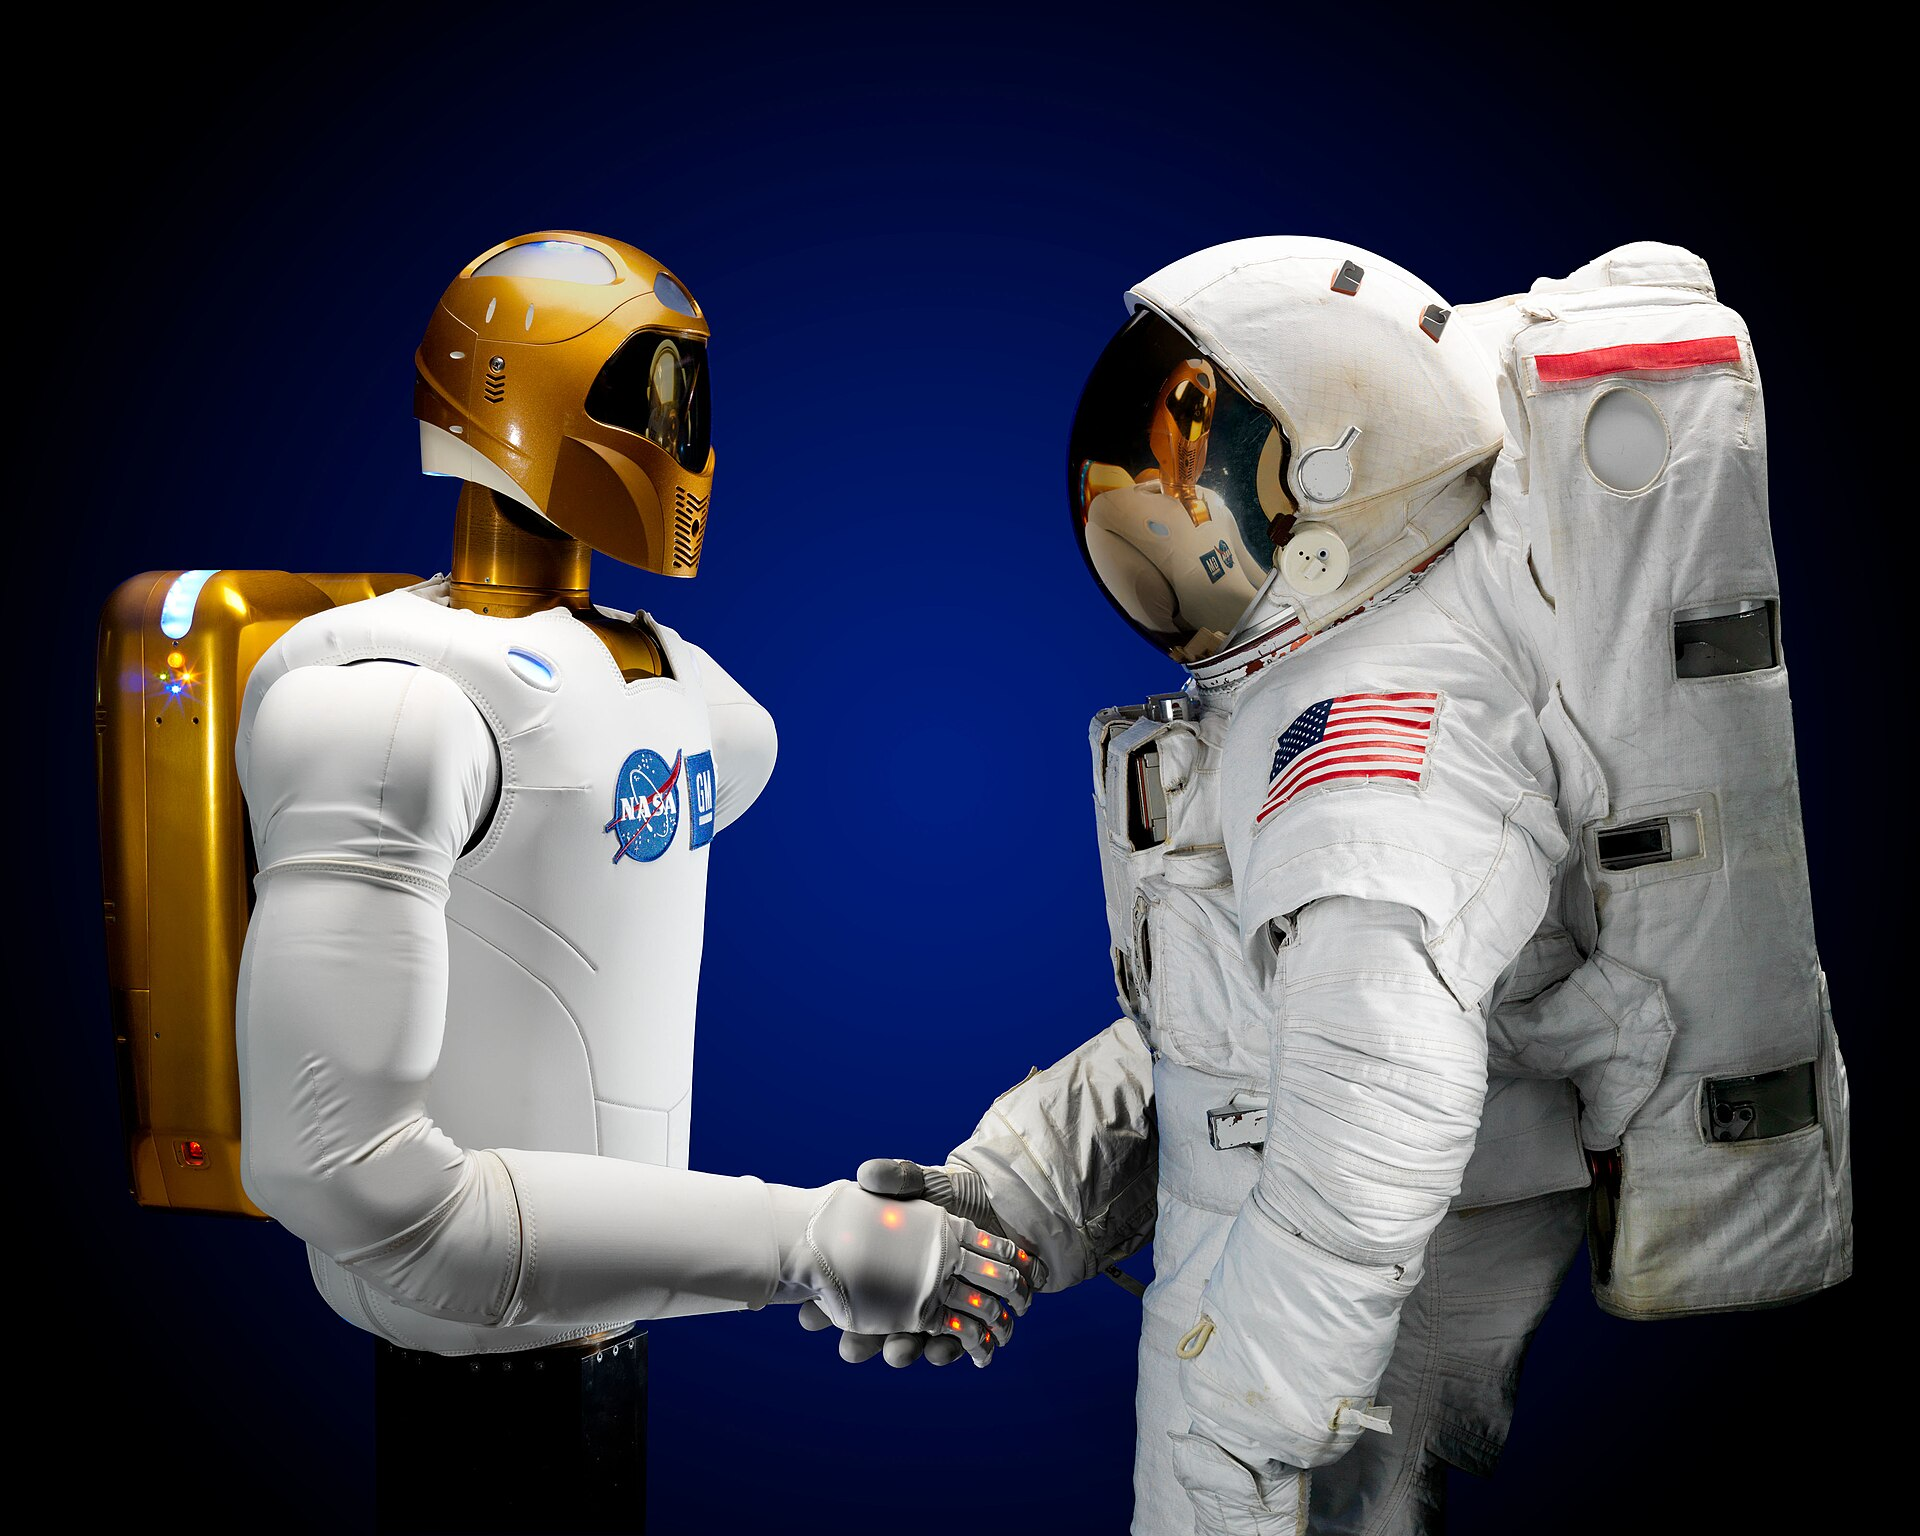
\includegraphics[width=\linewidth]{images/robonaut_handshake.jpg}
  \end{columns}
  \note{Agents built on LLMs act for people in recommendation, negotiation and
  multi-agent assistants. When such agents interact, outcomes depend on whether
  they cooperate, which makes their cooperative behaviour a governance question.
  Refs: Park et al., UIST 2023 (generative agents); Dafoe et al., Nature 2021
  (cooperative AI); Hammond et al., arXiv 2025 (multi-agent risks); Han et al.,
  Phil Trans R Soc A 2026 (social physics in the age of AI).}
\end{frame}

% ---------------------------------------------------------------------------
\begin{frame}{How do we measure LLM cooperation?}
  \begin{itemize}
    \item Let LLMs play classical games, e.g.\ the prisoner's dilemma
    \bigskip
    \item Report \hb{one cooperation rate}, under \hb{one payoff matrix}
    \bigskip
    \item Report what agents did, not the rule behind it
  \end{itemize}
  \vspace{0.8cm}
  \begin{center}
    \hq{\large Is a cooperation rate a property of the model,\\
      or of how the game is written down?}
  \end{center}
  \note{Prior work: Akata et al., Nature Human Behaviour 2025 (retaliation);
  Fontana et al., ICWSM 2025 (forgiveness); Lore and Heydari, Sci Rep 2024
  (game structure vs framing); our FAIRGAME, ECAI 2025 (language). They share
  two habits: one payoff matrix per model, and outcomes rather than decision
  rules.}
\end{frame}

% ---------------------------------------------------------------------------
\begin{frame}{The (iterated) prisoner's dilemma}
  \begin{columns}[T]
    \column{0.50\textwidth}
    \centering
    \card[2.1cm]{Cooperate}{pays a cost so both do better}\hspace{0.15cm}%
    \card[2.1cm]{Defect}{exploits, or avoids being exploited}\\[0.5cm]
    {\mdseries\small
    \renewcommand{\arraystretch}{1.35}
    \begin{tabular}{c|cc}
      & \bfseries C & \bfseries D\\ \hline
      \bfseries C & $R,\,R$ & $S,\,T$\\
      \bfseries D & $T,\,S$ & $P,\,P$
    \end{tabular}}\\[0.25cm]
    {\small $T > R > P > S$}
    \column{0.50\textwidth}
    A \hb{strategy} maps the history to the next move\par
    \medskip
    \begin{itemize}
      \item \sAllC: always cooperate
      \item \sAllD: always defect
      \item \sTFT: copy the partner
      \item \sWSLS: win-stay, lose-shift
    \end{itemize}
    \vspace{0.25cm}
    \centering
    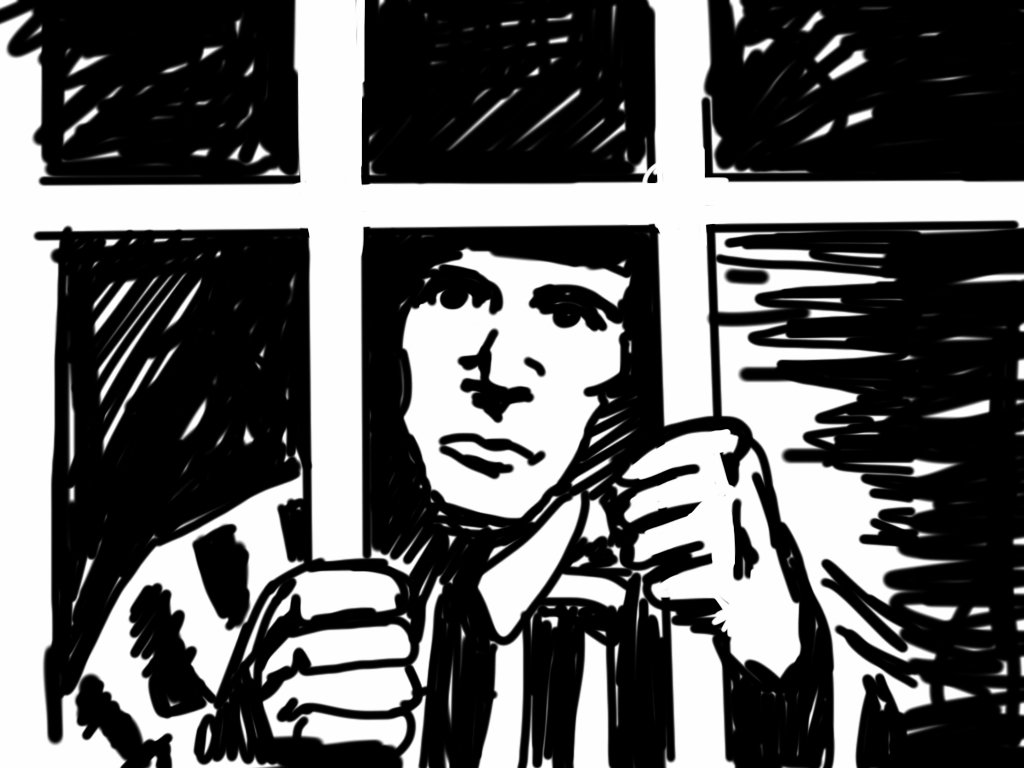
\includegraphics[height=2.4cm]{images/prisoner_sketch.jpg}
  \end{columns}
  \note{Background. Defection dominates, yet mutual cooperation beats mutual
  defection. Stress the strategy view: a strategy maps history to the next move;
  the four canonical memory-one rules are the vocabulary used later to read LLM
  trajectories. Refs: Axelrod and Hamilton, Science 1981; Nowak and Sigmund,
  Nature 1993; Han, Pereira and Santos, Artificial Life 2012.}
\end{frame}

% ---------------------------------------------------------------------------
\begin{frame}{Same game, different units}
  \begin{columns}[T]
    \column{0.68\textwidth}
    \begin{itemize}
      \item Multiply every payoff by $\lam > 0$
      \bigskip
      \item Preferences, best replies, Nash equilibria and replicator orbits
        are all \hb{unchanged}
      \bigskip
      \item Cents, dollars or thousands of pounds: the same game
    \end{itemize}
    \column{0.30\textwidth}
    \centering
    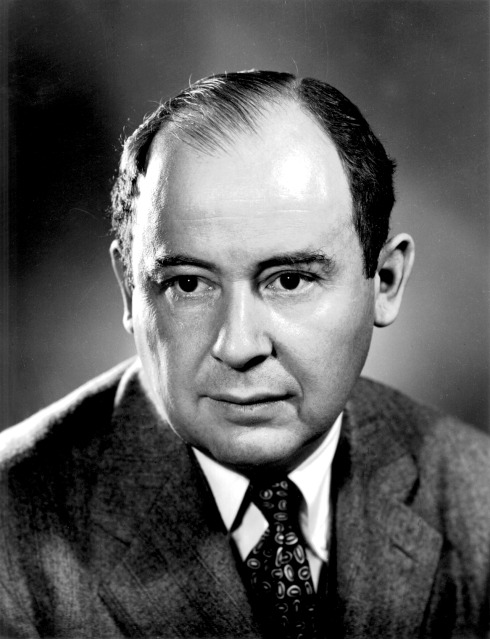
\includegraphics[width=0.92\linewidth]{logos/vonneumann.jpg}\par
    {\scriptsize\bfseries John von Neumann\par}
    {\mdseries\tiny von Neumann \& Morgenstern,\\ \emph{Theory of Games}, 1944\par}
  \end{columns}
  \vspace{0.4cm}
  \punch{Predicted effect of $\lam$ on a rational agent: exactly zero}
  \note{A positive affine transformation of a von Neumann-Morgenstern utility
  (von Neumann and Morgenstern, Theory of Games and Economic Behavior, 1944;
  the expected-utility axioms appear in the 2nd edition, 1947; Luce and Raiffa
  1957). "Rational agent" here means an agent whose whole utility is the stated
  payoffs. In the replicator
  dynamics only time is rescaled (backup slide: vector fields at lambda 0.01 and
  1000 agree to 4e-14). Why it is a sharp test: prompt order, formatting and
  persona have no defined null, payoff rescaling does. To our knowledge, the
  first such test across many models and languages. Caveat: the null is for an
  agent whose whole utility is the stated payoffs; narrative and persona text do
  not scale with lambda. Human stake effects exist but are modest and need
  stakes large relative to income (Camerer and Hogarth 1999; Kocher et al.
  2008).}
\end{frame}

% ---------------------------------------------------------------------------
\begin{frame}{Research questions}
  \begin{enumerate}
    \item Is LLM behaviour \hb{invariant} to rescaling the payoffs?
    \bigskip\bigskip
    \item Does it depend on the \hb{language} and the \hb{persona}?
    \bigskip\bigskip
    \item Does rescaling change only how often a model cooperates,
      or also its \hb{strategy}?
  \end{enumerate}
\end{frame}

% ===========================================================================
% 2. Experimental design
% ===========================================================================
\begin{frame}{Experimental design}
  \begin{columns}[c]
    \column{0.55\textwidth}
    \centering
    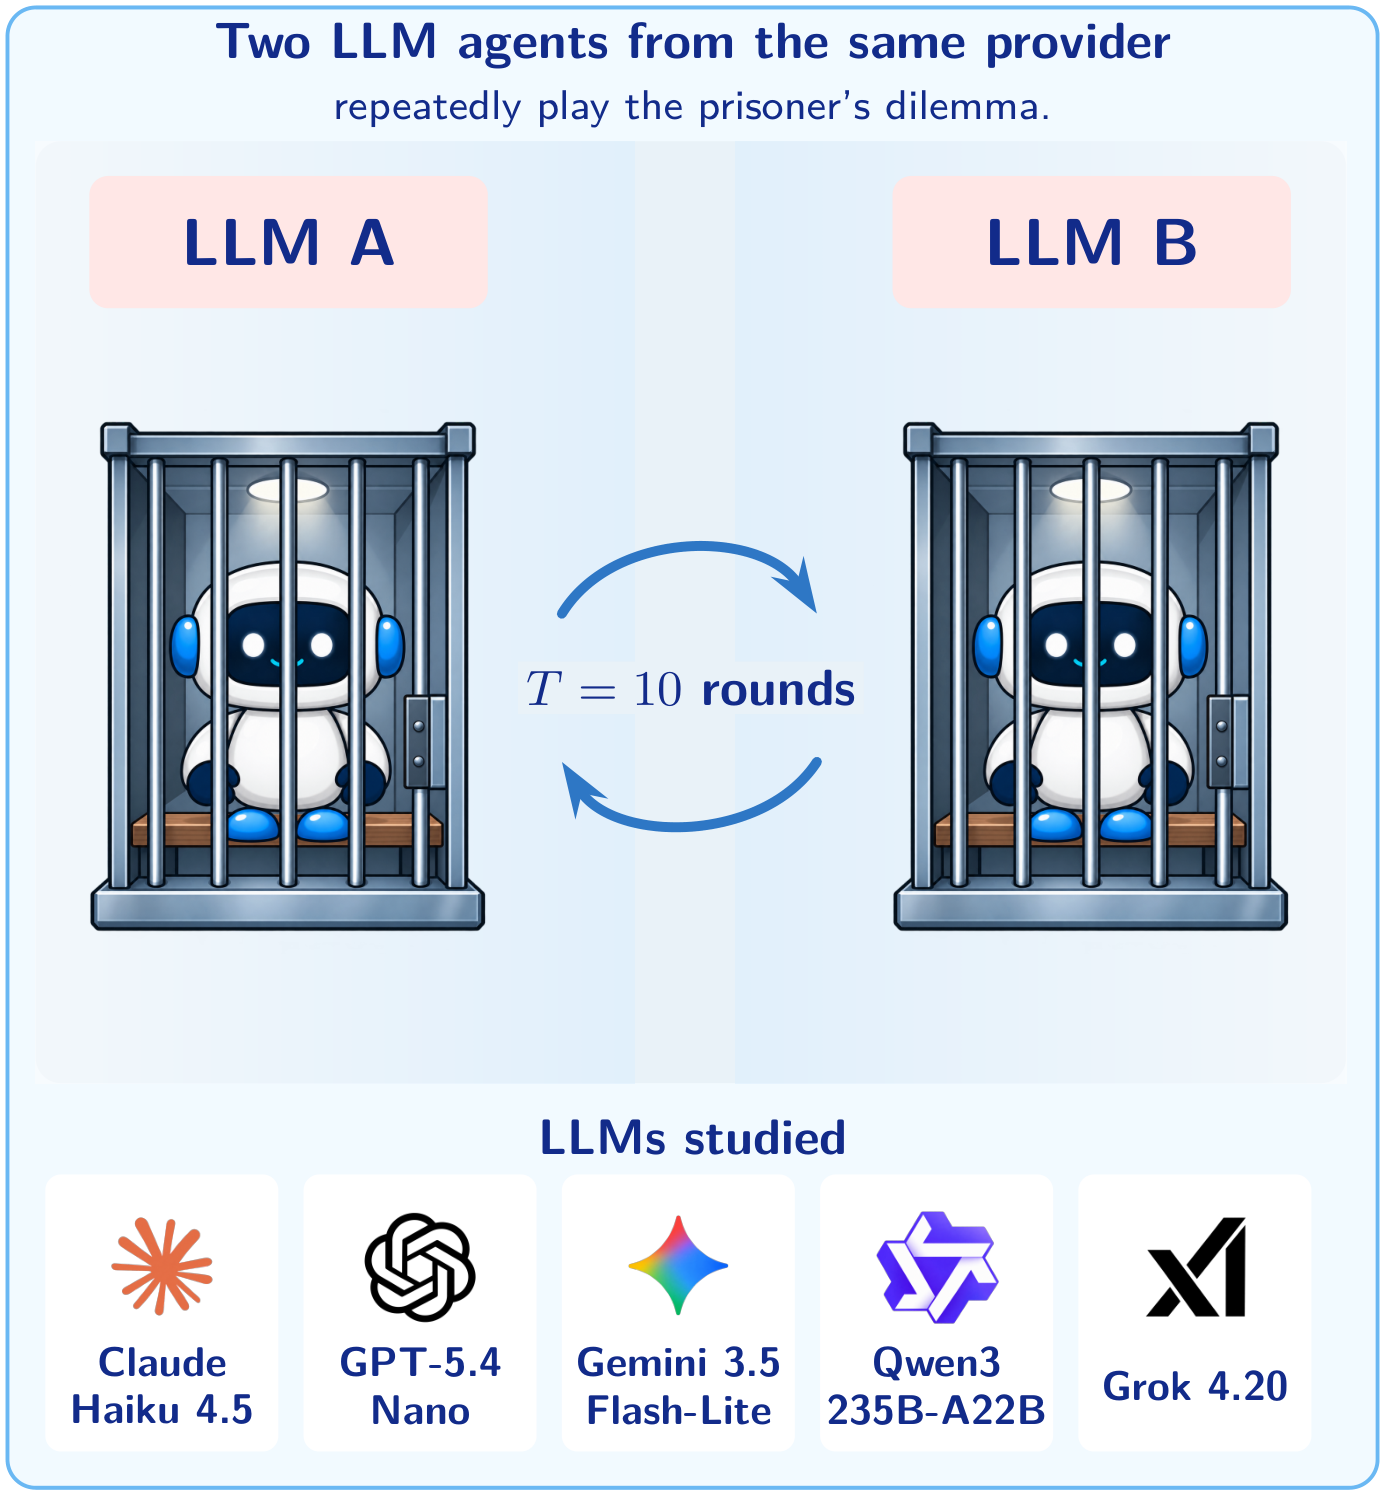
\includegraphics[height=6.6cm]{figures/overview_left.png}
    \column{0.43\textwidth}
    \begin{itemize}
      \item Two agents of the \hb{same model} play each other
      \bigskip
      \item 10 rounds of the prisoner's dilemma
      \bigskip
      \item Every payoff multiplied by $\lam$
    \end{itemize}
  \end{columns}
  \note{Left half of the paper's Figure 1. Two agents from the same provider
  play ten rounds of the prisoner's dilemma; the payoff matrix is multiplied by
  lambda. Grid: 5 models x 10 scales x 5 languages x 4 persona pairings x 10
  replicates.}
\end{frame}

% ---------------------------------------------------------------------------
\begin{frame}{The payoff-scaled prisoner's dilemma}
  \begin{columns}[c]
    \column{0.58\textwidth}
    \begin{itemize}
      \item FAIRGAME\fn{1} scenario: a \hb{criminal interrogation}
      \medskip
      \item Penalties to minimise
    \end{itemize}
    \column{0.40\textwidth}
    \centering
    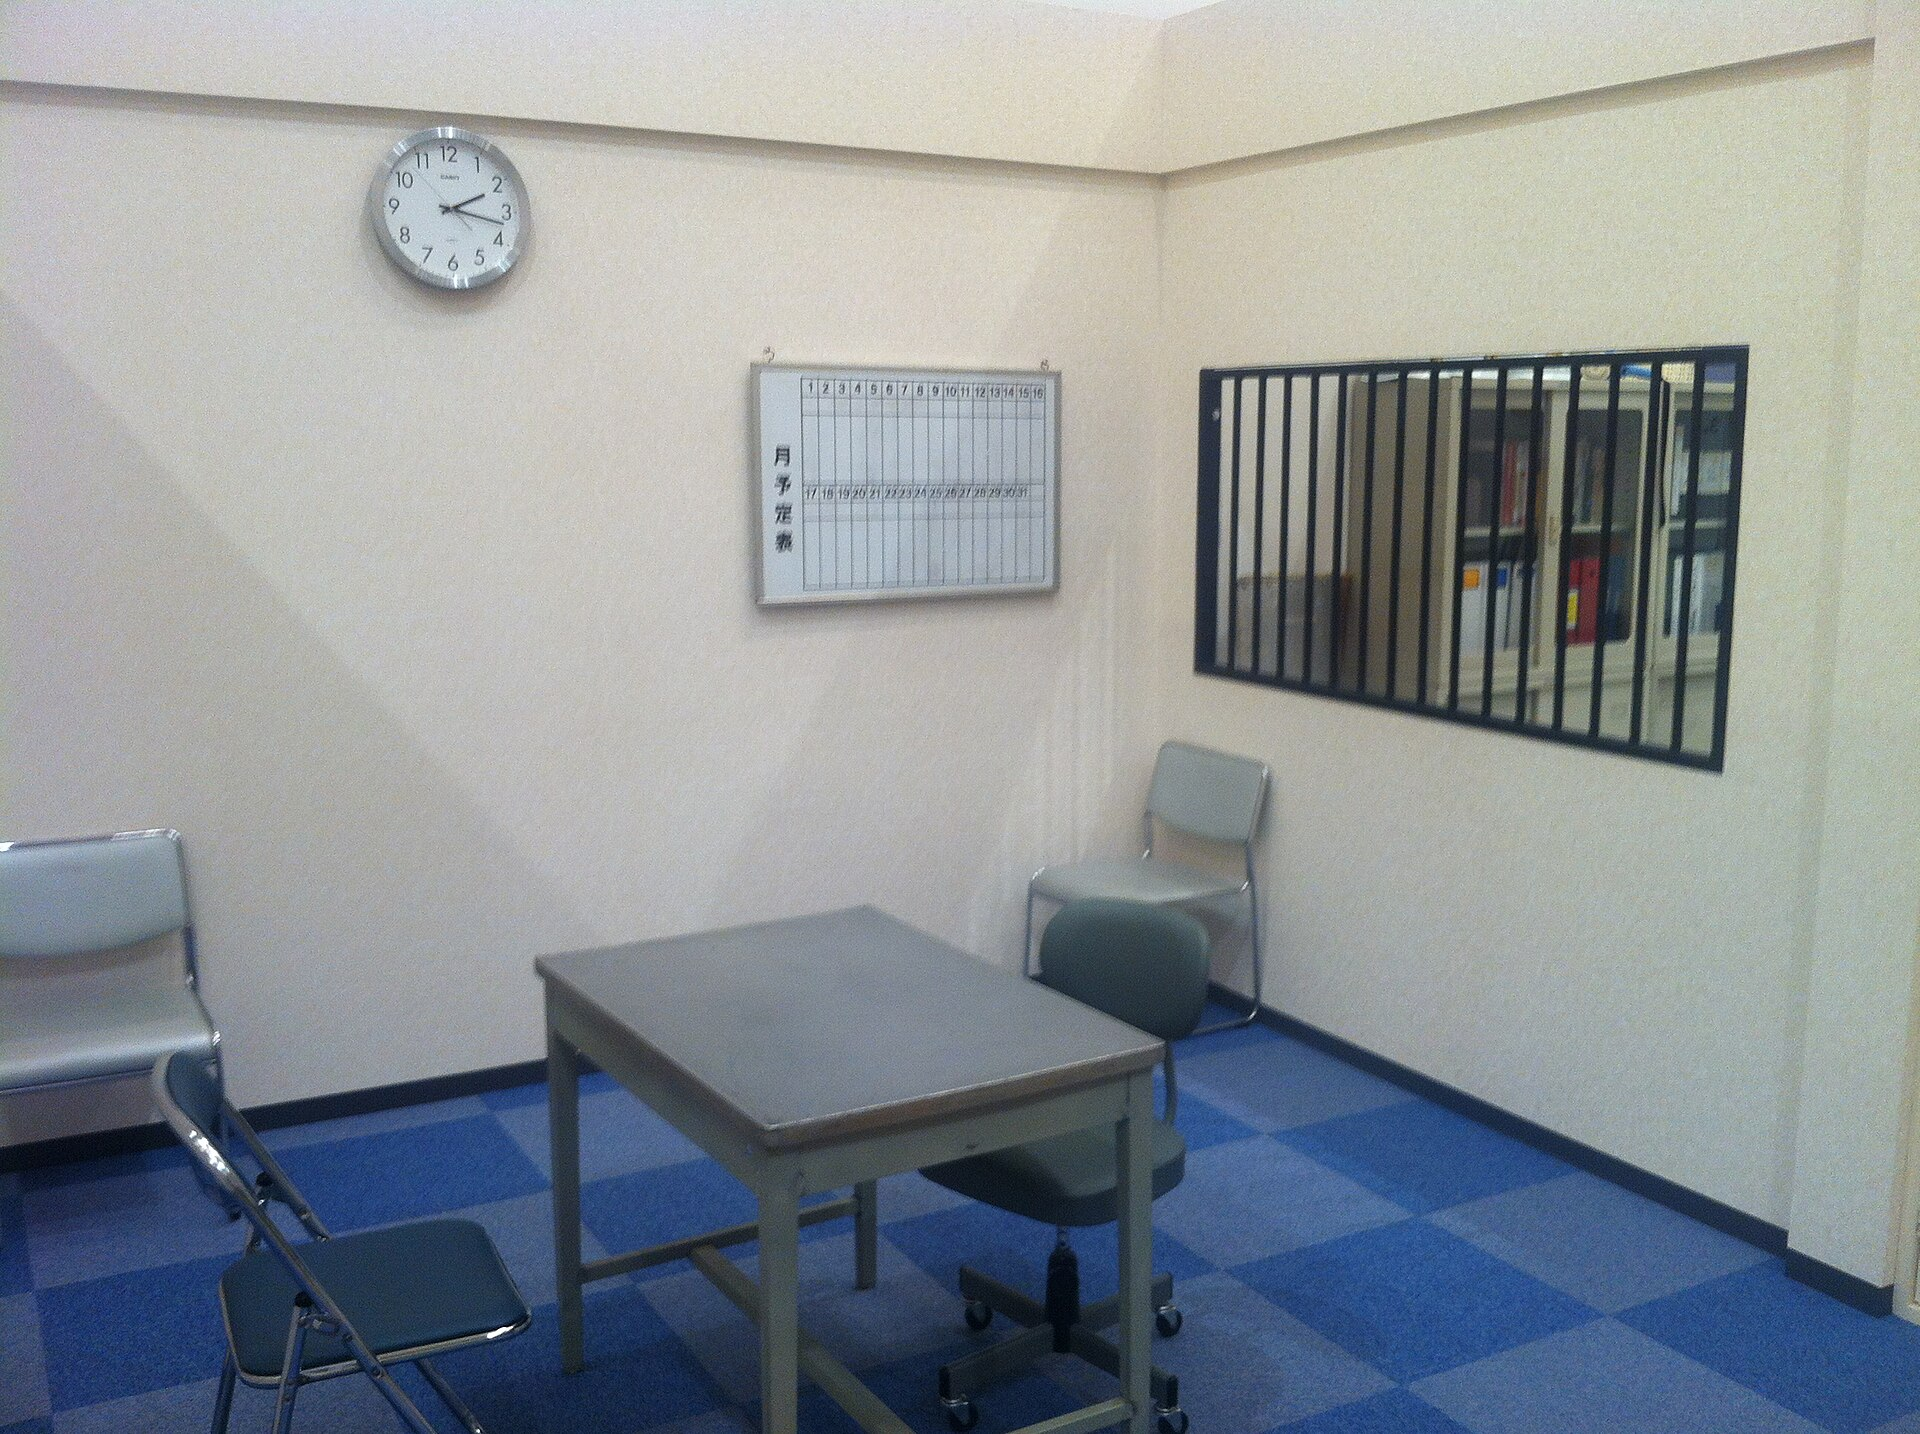
\includegraphics[height=2.25cm]{images/interrogation_room.jpg}
  \end{columns}
  \vspace{0.3cm}
  \centering
  {\mdseries\footnotesize
  \renewcommand{\arraystretch}{1.3}
  \begin{tabular}{c|cc}
    \multicolumn{3}{c}{\bfseries $\lam = 0.1$}\\[1pt]
    & A & B\\ \hline
    A & $0.6,\,0.6$ & $0,\,1.0$\\
    B & $1.0,\,0$ & $0.2,\,0.2$
  \end{tabular}\hspace{0.35cm}
  \begin{tabular}{c|cc}
    \multicolumn{3}{c}{\bfseries $\lam = 1$}\\[1pt]
    & A & B\\ \hline
    A & $6,\,6$ & $0,\,10$\\
    B & $10,\,0$ & $2,\,2$
  \end{tabular}\hspace{0.35cm}
  \begin{tabular}{c|cc}
    \multicolumn{3}{c}{\bfseries $\lam = 10$}\\[1pt]
    & A & B\\ \hline
    A & $60,\,60$ & $0,\,100$\\
    B & $100,\,0$ & $20,\,20$
  \end{tabular}}\par
  \vspace{0.35cm}
  \raggedright
  \begin{itemize}
    \item Option A = defect, Option B = cooperate
    \medskip
    \item Ten scales, five orders of magnitude:\\[2pt]
      $\lam \in \{0.01,\ 0.1,\ 0.25,\ 0.5,\ 1,\ 2,\ 5,\ 10,\ 100,\ 1000\}$
  \end{itemize}
  \slidefoot{1}{Buscemi, Proverbio, Di Stefano, Han, Castignani, Li\`o.
    \textbf{FAIRGAME: a framework for AI agents bias recognition using game theory}. ECAI, 2025.}
  \note{FAIRGAME prompt: a criminal interrogation, penalties to minimise,
  Options A and B, running history, announced horizon of 10 rounds. Option A
  lowers the penalty in both columns, so it is the dominant (defecting) action.
  Penalties T=0 < R=2 < P=6 < S=10 are the prisoner's dilemma on u = -penalty.
  At lambda <= 0.1 (sub-unit) no payoff shown exceeds 1. Logs confirm the
  polarity: own cooperation vs own utility rho = -0.015, partner cooperation
  rho = +0.916, welfare vs joint cooperation rho = +0.985.}
\end{frame}

% ---------------------------------------------------------------------------
\begin{frame}{Models, languages, personas}
  \begin{columns}[c]
    \column{0.64\textwidth}
    \begin{itemize}
      \item \hb{5 models}, each playing itself\\
        {\mdseries\small Claude Haiku 4.5, GPT-5.4 Nano, Gemini 3.5 Flash-Lite,
         Qwen3 235B-A22B, Grok 4.20}
      \medskip
      \item \hb{5 languages}\\
        {\mdseries\small English, French, Vietnamese, Chinese, Arabic}
      \medskip
      \item \hb{2 personas}\\
        {\mdseries\small\itshape ``You are cooperative.''\\ ``You are selfish.''}
      \medskip
      \item 10 rounds, simultaneous moves
    \end{itemize}
    \column{0.34\textwidth}
    \centering
    \begin{tikzpicture}[font=\titlefont\mdseries\small]
      \node[hi=cBlu] at (0,0)      {Hello};
      \node[hi=cPea] at (1.75,0)   {Bonjour};
      \node[hi=cGrn] at (0.15,-0.75){Xin chào};
      \node[hi=cSan] at (1.75,-0.75){{\zhfont 你好}};
      \node[hi=cLav] at (0.95,-1.5){{\arfont\beginR مرحبا\endR}};
    \end{tikzpicture}\\[0.35cm]
    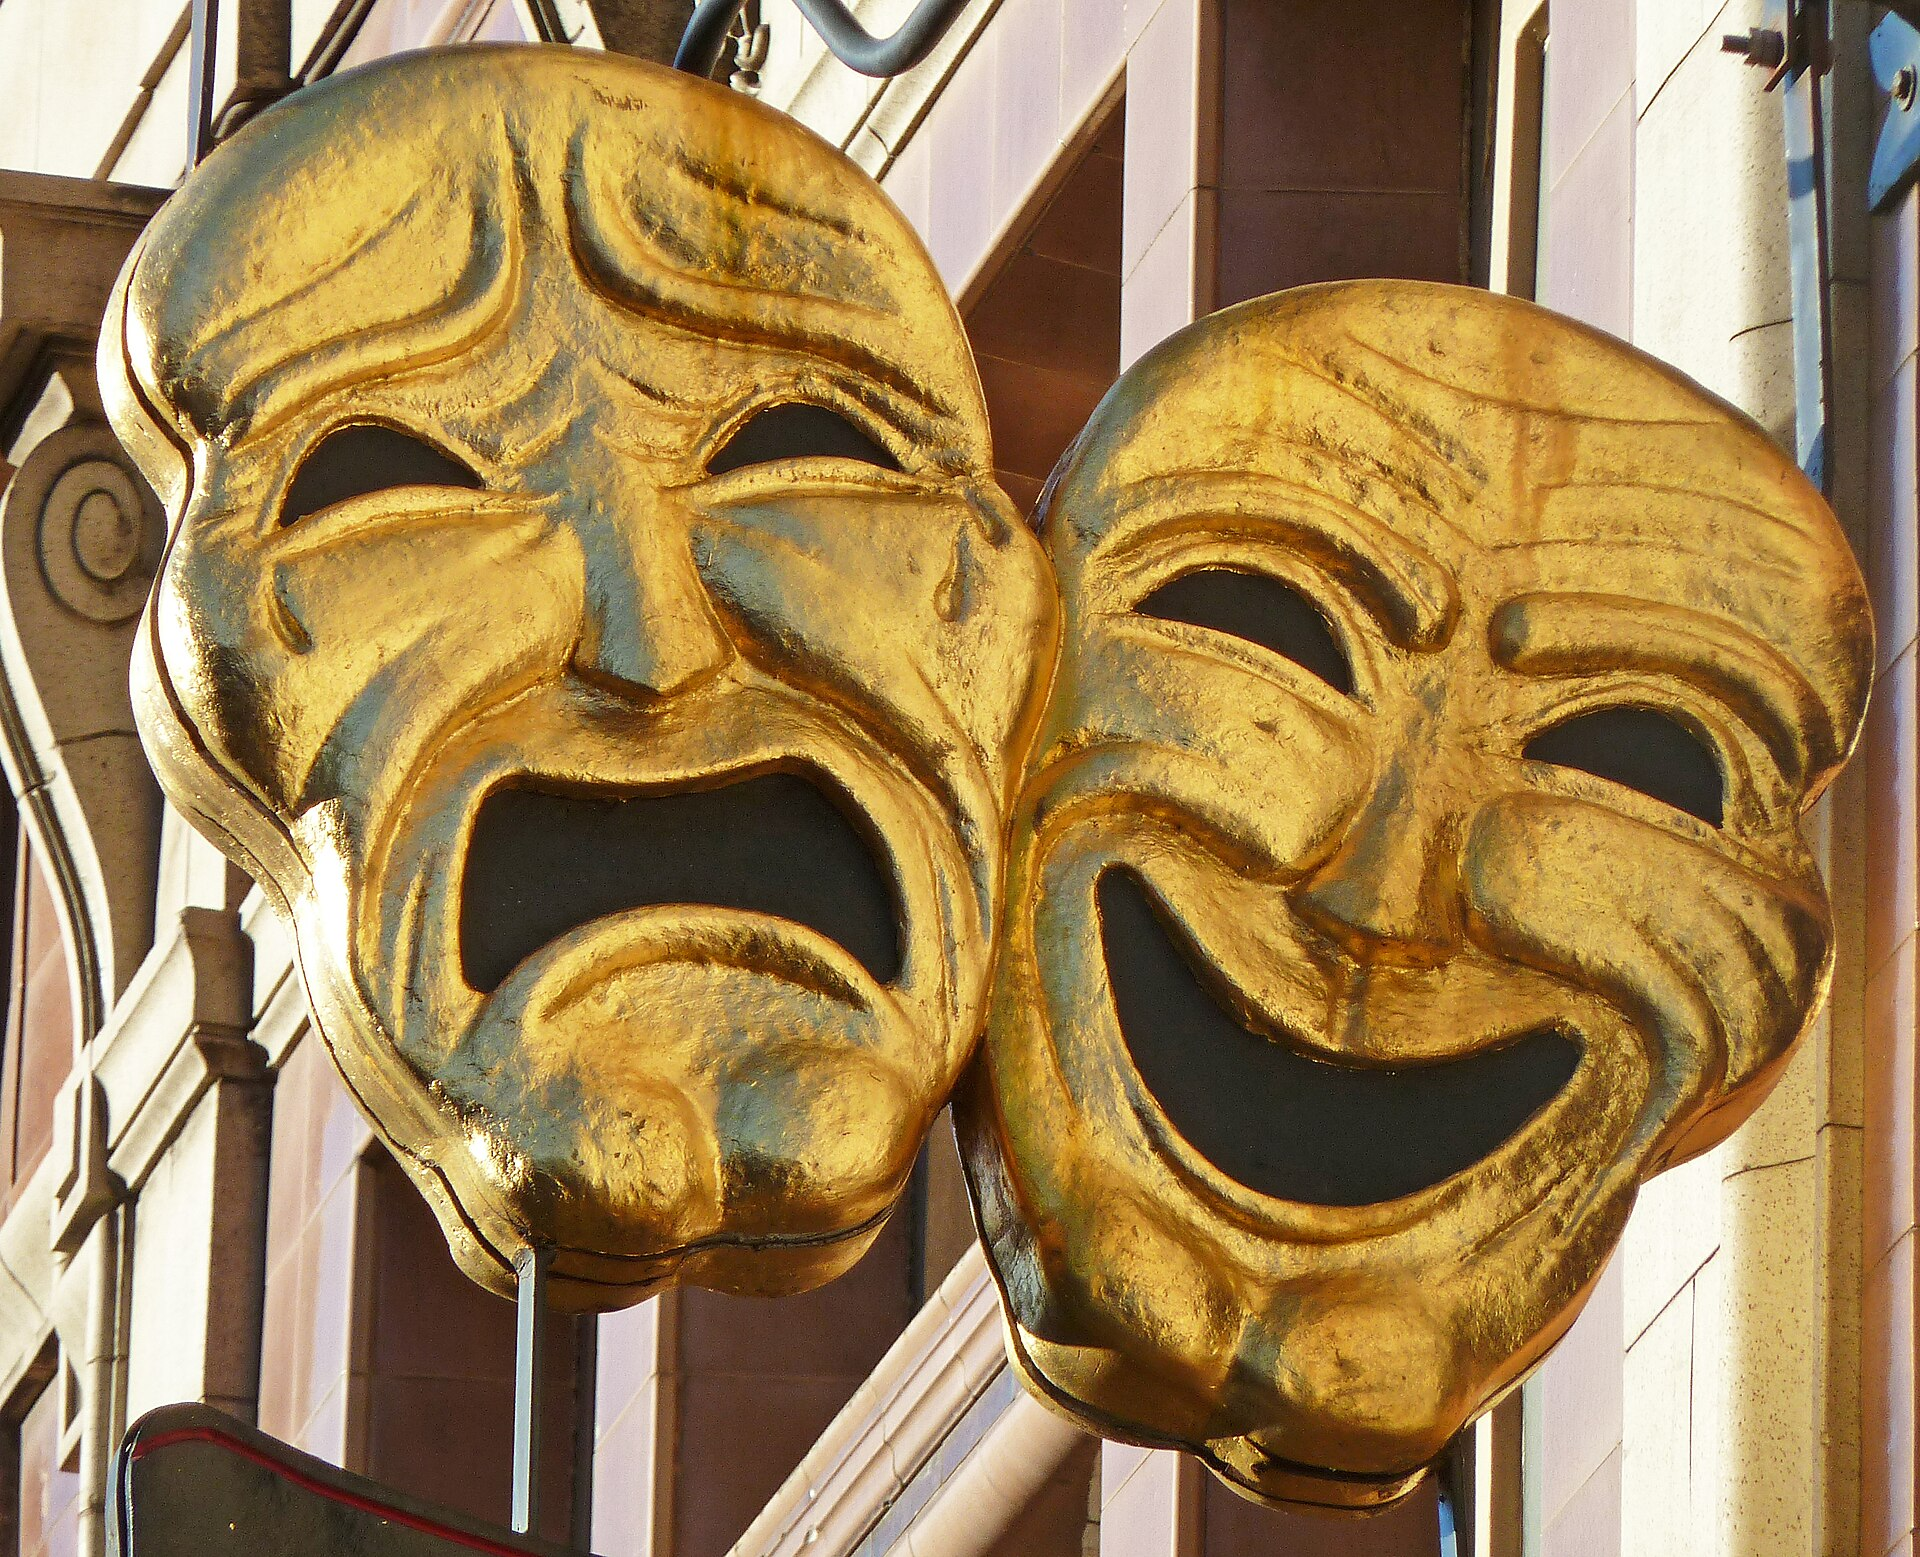
\includegraphics[width=0.62\linewidth]{images/persona_masks.jpg}
  \end{columns}
  \vspace{0.3cm}
  \begin{center}
    \setlength{\fboxsep}{5pt}
    \fcolorbox{TeesOrange}{white}{\begin{minipage}{0.7\linewidth}\centering
      10,000 games\ \ $\cdot$\ \ 200,000 decisions\end{minipage}}
  \end{center}
  \note{Persona is Latin for a theatre mask. Templates byte-identical to FAIRGAME. Four ordered persona pairings x
  10 replicates; the opponent's persona is never disclosed. Free-text replies;
  unparseable after 3 tries is recorded as defection (at most 2 percent per
  run), so it can only push cooperation down. The grid is exactly balanced
  (enforced by a build-time guard): 200 dyads, 400 agent-games per model x
  scale cell; 20,000 agent-games in all. Whole study cost under US\$160.}
\end{frame}

% ---------------------------------------------------------------------------
\begin{frame}{Strategy read-out\fn{2}}
  \centering
  \begin{tikzpicture}[font=\titlefont\mdseries\small]

    % ---- training: synthetic play -> LSTM ---------------------------------
    \node[ell=cYel, minimum width=1.85cm, minimum height=1.25cm] (syn) at (0.95,0)
      {Synthetic\\games};
    \node[box=cBlu, fill=cBlu!35, minimum width=1.05cm, minimum height=2.2cm,
          rounded corners=5pt, font=\titlefont\bfseries\small] (str) at (4.35,0) {\sAllC\\[2pt]\sAllD\\[2pt]\sTFT\\[2pt]\sWSLS};
    \node[lab, below=1pt of str] {Strategies};
    % the fan is drawn before the noise node, so the node sits on top of it
    \draw[fan] (syn.25)  -- ([yshift= 0.85cm]str.west);
    \draw[fan] (syn.8)   -- ([yshift= 0.30cm]str.west);
    \draw[fan] (syn.-8)  -- ([yshift=-0.30cm]str.west);
    \draw[fan] (syn.-25) -- ([yshift=-0.85cm]str.west);
    \node[ell=cPea, minimum width=1.2cm, minimum height=0.9cm,
          font=\titlefont\mdseries\scriptsize] (noi) at (2.65,0) {Noise\\0, 5\%};
    \draw[big] (5.05,0) -- (6.05,0) node[lab, midway, above=4pt] {Training};
    \node[box=cLav, minimum width=1.7cm, minimum height=1.0cm] (lstm) at (7.10,0) {LSTM};

    % ---- inference: an LLM game -> rule base -> label ---------------------
    \node[ell=cYel, minimum width=1.85cm, minimum height=1.25cm] (llm) at (0.95,-3.05)
      {LLM game\\(10 rounds)};
    \draw[big] (1.95,-3.05) -- (3.15,-3.05) node[lab, midway, above=4pt] {Match};
    \begin{scope}[every node/.append style={font=\titlefont\mdseries\footnotesize,
                  text width=1.42cm, inner sep=2pt, minimum height=1.1cm}]
      \node[box=cGrn] (ded) at (4.12,-3.05) {Deduced\\{\scriptsize one fits}};
      \node[box=cSan] (amb) at (5.72,-3.05) {Ambiguous\\{\scriptsize several fit}};
      \node[box=cPea] (unm) at (7.32,-3.05) {Unmatched\\{\scriptsize none fits}};
    \end{scope}
    \draw[dashed, line width=0.9pt] (3.25,-2.38) rectangle (8.19,-3.72);
    \node[lab] at (5.72,-4.02) {Canonical rule base};
    \draw[thin] ([xshift=-0.45cm]lstm.south) -- (amb.north)
      node[pos=0.72, left=2pt, align=right, font=\titlefont\mdseries\scriptsize]
      {ranks within\\the set};
    \draw[thin] ([xshift=0.2cm]lstm.south) -- (unm.north)
      node[pos=0.72, right=2pt, align=left, font=\titlefont\mdseries\scriptsize]
      {decides\\alone};
    \draw[big] (8.33,-3.05) -- (9.78,-3.05) node[lab, midway, above=4pt] {Inference};
    \node[box=cPnk, minimum width=1.7cm, minimum height=1.25cm,
          rounded corners=6pt] (out) at (10.66,-3.05) {Resembled\\strategy};
  \end{tikzpicture}\par
  \vspace{0.35cm}
  \punch{Resembles, not plays}
  \slidefoot{2}{Di Stefano, Jayne, Angione, Han. \textbf{Recognition of behavioural
    intention in repeated games using machine learning}. ALIFE, 2023.}
  \note{Adapted from the intention-recognition pipeline of Di Stefano, Jayne,
  Angione and Han (ALIFE 2023); see also Han, Pereira and Santos (Artificial
  Life 2012). Top row: the LSTM is trained on synthetic AllC, AllD, TFT and WSLS
  play only, at 0 and 5 percent execution noise; no LLM transcript is used.
  Bottom row: each 10-round LLM game is first matched exactly against the four
  rules. Deduced games keep their rule; for ambiguous games the LSTM ranks
  within the matching set, so it never overturns a deduction; only unmatched
  games are labelled by the LSTM alone. Accuracy: 98.5 percent in distribution,
  93.6 percent at held-out 10 percent noise. A label-free companion measure:
  rounds violating the nearest rule.}
\end{frame}

% ===========================================================================
% 3. Results
% ===========================================================================
\begin{frame}{Every model violates scale invariance}
  \centering
  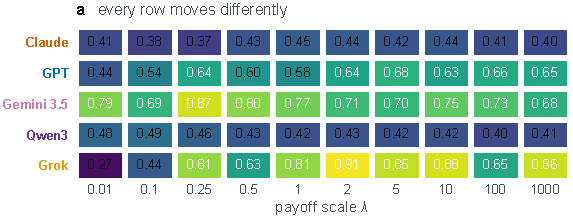
\includegraphics[width=\linewidth]{figures/f_landscape_a.pdf}\par
  {\footnotesize\mdseries Each tile: cooperation rate, the share of rounds
    played C (400 agent-games)\par}
  \vspace{0.35cm}
  \raggedright
  \begin{itemize}
    \item Theory predicts flat rows: \hb{every row moves}
    \medskip
    \item Grok: 0.27 at $\lam = 0.01$, 0.91 at $\lam = 2$
  \end{itemize}
  \note{Mean cooperation per model and scale, 400 agent-games per cell.
  Permutation test on the scale label: p <= 0.0025 for every model; per-model
  Wald chi-square on 9 df, all p < 0.001. Ranges: Claude 0.081, GPT 0.243,
  Gemini 0.190, Qwen 0.095, Grok 0.636 (backup table). Largest departures sit at
  the low-payoff end.}
\end{frame}

% ---------------------------------------------------------------------------
\begin{frame}{Five models, five machine characters}
  \centering
  \vspace{0.3cm}
  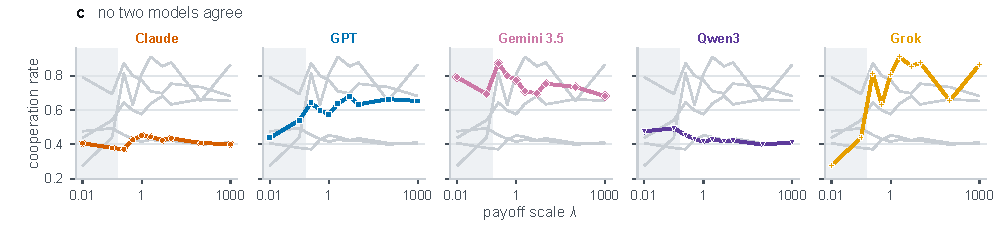
\includegraphics[width=\linewidth]{figures/f_landscape_c.pdf}\par
  \vspace{0.7cm}
  \raggedright
  \begin{itemize}
    \item Up, down, dip, jump: each model has its own response
    \medskip
    \item No single universal pattern
  \end{itemize}
  \note{Grey lines are the other four models; shaded band is the sub-unit
  regime. Grok defects at micro-stakes and cooperates at standard stakes. GPT
  climbs from 0.44 and saturates near 0.65. Claude dips at lambda = 0.25
  (0.37) and recovers (0.45 at lambda 1). Gemini stays highly cooperative but
  drifts down (0.87 to 0.68). Qwen becomes slightly less cooperative (0.49 to
  0.40).}
\end{frame}

% ---------------------------------------------------------------------------
\begin{frame}{Pooling across models hides the effect}
  \centering
  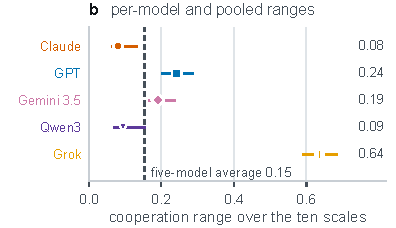
\includegraphics[width=0.66\linewidth]{figures/f_landscape_b.pdf}\par
  \vspace{0.3cm}
  \raggedright
  \begin{itemize}
    \item The average moves less than three of the five models
    \item Model $\times$ scale: three times the variance of scale alone
  \end{itemize}
  \punch{The average describes no real model}
  \note{Pooled range 0.154 vs mean within-model range 0.249 (attenuation 1.62);
  6 of 10 model pairs are anticorrelated, so curves cancel. Type-II ANOVA on 250
  cell means: model x scale 17.9 percent vs scale main effect 5.8 percent
  (backup). Without Grok the scale main effect is not significant
  (F(9,108) = 1.15, p = 0.33), yet each remaining model still moves. Not a power
  problem: more data only tightens the interval around an average that
  describes no model.}
\end{frame}

% ---------------------------------------------------------------------------
\begin{frame}{Remark\fn{3}}
  \begin{itemize}
    \item Rescaling the payoffs, an inert change of units in theory, moves
      cooperation in every model
    \bigskip
    \item The response is model-specific in size, shape and direction
    \bigskip
    \item Averages over models conceal it
  \end{itemize}
  \slidefoot{3}{Han, Huynh, Duy-Minh, \dots, Buscemi, Trang. \textbf{Payoff scaling
    shapes cooperation in LLM agents across languages}. arXiv:2601.19082, 2026.}
\end{frame}

% ---------------------------------------------------------------------------
\begin{frame}{Scale sensitivity depends on language}
  \centering
  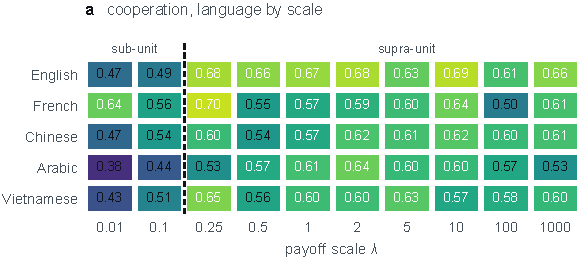
\includegraphics[width=\linewidth]{figures/f_language_a.pdf}\par
  \vspace{0.4cm}
  \raggedright
  \begin{itemize}
    \item Within a model, sensitivity differs about two-fold between languages
    \medskip
    \item English is the most scale-sensitive language for 4 of 5 models
  \end{itemize}
  \note{Cooperation pooled over the five models; dashed line separates the
  sub-unit and supra-unit regimes. Across model-language cells sensitivity
  differs by an order of magnitude; the most cooperative language differs by
  model. Caveat: the Arabic and Chinese templates state penalties but phrase
  the goal as maximising a reward, so language is partly confounded with
  template wording. Read this as a prompt-stimulus by scale interaction, not a
  cultural mechanism. Within-language comparisons are clean.}
\end{frame}

% ---------------------------------------------------------------------------
\begin{frame}{Payoff scale flips the persona instruction}
  \begin{columns}[c]
    \column{0.62\textwidth}
    \centering
    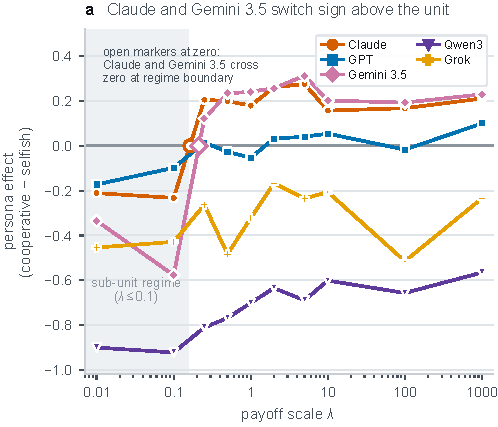
\includegraphics[width=\linewidth]{figures/f_persona_a.pdf}
    \column{0.36\textwidth}
    \begin{itemize}\small
      \item At $\lam \le 0.1$, all five models cooperate \hb{more} when told
        \emph{``You are selfish''}
      \medskip
      \item Claude and Gemini flip sign above it
      \medskip
      \item Qwen and Grok: inverted at every scale
    \end{itemize}
  \end{columns}
  \note{Persona effect = cooperation under the cooperative persona minus under
  the selfish one. Sub-unit vs supra-unit: Claude -0.22 to +0.21, Gemini -0.46
  to +0.22 (sign flips); GPT -0.14 to +0.02, not significant (abolished, not
  reversed); Qwen -0.91 to -0.68; Grok -0.44 to -0.30. Descriptive: we do not
  identify why the instruction changes direction. Role prompts need checking
  across payoff contexts.}
\end{frame}

% ---------------------------------------------------------------------------
\begin{frame}{Payoff scale changes the strategy mix}
  \centering
  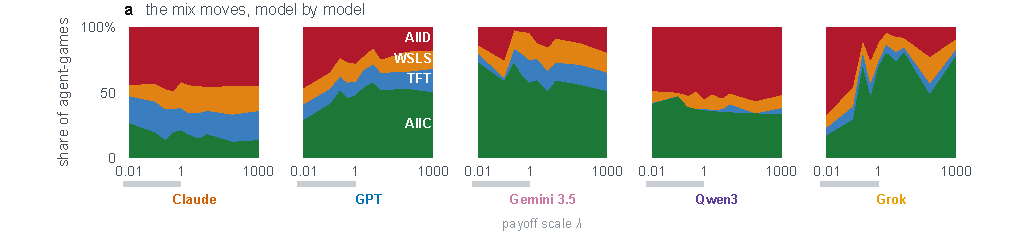
\includegraphics[width=\linewidth]{figures/f_strategy_mix_a.pdf}\par
  \vspace{0.3cm}
  \begin{columns}[c]
    \column{0.55\textwidth}
    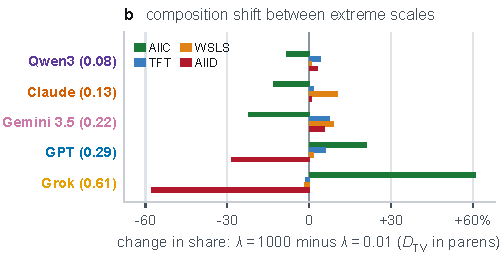
\includegraphics[width=\linewidth]{figures/f_strategy_mix_b.pdf}
    \column{0.43\textwidth}
    \begin{itemize}
      \item GPT: AllD $\to$ AllC
      \medskip
      \item Grok: complete reversal
    \end{itemize}
  \end{columns}
  \note{Two models with the same cooperation rate can play very differently.
  Panel b: change in label share between lambda 1000 and 0.01, total variation
  distance in brackets. Gemini: AllC gives way to TFT-like and WSLS-like play.}
\end{frame}

% ---------------------------------------------------------------------------
\begin{frame}{Strategy labels are resemblances}
  \centering
  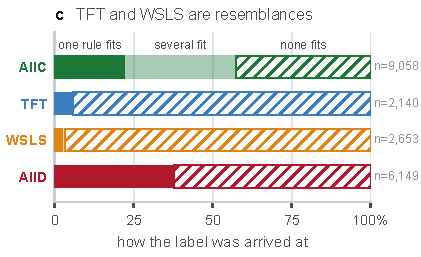
\includegraphics[width=0.72\linewidth]{figures/f_strategy_mix_c.pdf}\par
  \vspace{0.5cm}
  \raggedright
  \begin{itemize}
    \item 95\% of TFT and 97\% of WSLS labels fit \hb{no rule} exactly
    \medskip
    \item As stakes grow, play drifts away from the textbook rules in most models
  \end{itemize}
  \note{Exact figures: 94.6 percent of TFT and 97.1 percent of WSLS labels are
  attributions on unmatched play. Share matched by exactly one rule falls with
  lambda in 4 of 5 models (Qwen 72 to 54 percent, Claude 18 to 4). Rounds
  violating the nearest rule rise with lambda, a label-free measure; Grok is the
  exception, moving towards pure-policy play. So a rising TFT share is not
  adoption of Tit-for-Tat.}
\end{frame}

% ---------------------------------------------------------------------------
\begin{frame}{Where payoff scale does matter}
  \begin{itemize}
    \item Finite populations with \hb{social imitation}:
  \end{itemize}
  \[ P(i \to j) = \frac{1}{1 + e^{-\beta\lam\,(\pi_j - \pi_i)}} \]
  \begin{itemize}
    \item Raising the stakes $=$ raising the intensity of selection
  \end{itemize}
  \centering
  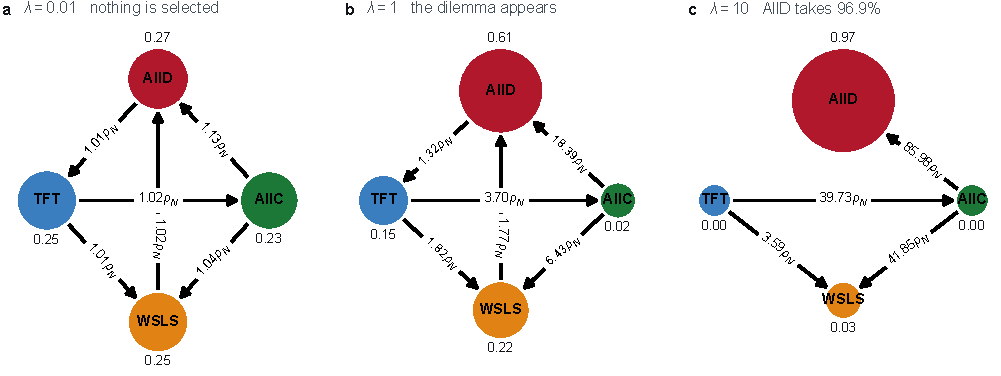
\includegraphics[width=\linewidth]{figures/f_invasion.pdf}
  \note{Pairwise Fermi rule, population Z = 100, rare mutations, beta = 0.1,
  error 0.05, 10 rounds; pi are the unscaled payoffs. Node area: stationary
  probability; edges: fixation in multiples of neutral drift 1/Z. At lambda 0.01
  nothing is selected; at lambda 10 AllD takes 96.9 percent. Refs: Nowak et al.,
  Nature 2004; Sigmund, The Calculus of Selfishness 2010.}
\end{frame}

% ---------------------------------------------------------------------------
\begin{frame}{Pooled LLM agents move the opposite way}
  \centering
  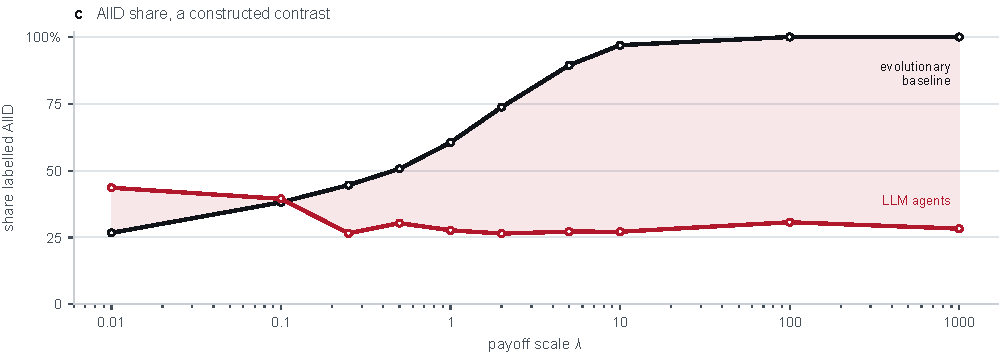
\includegraphics[width=\linewidth]{figures/f_egt_vs_llm_c.pdf}\par
  \vspace{0.4cm}
  \raggedright
  \begin{itemize}
    \item Evolutionary baseline: more AllD as stakes grow
    \medskip
    \item LLM agents, pooled over models: less AllD
  \end{itemize}
  \note{From lambda 0.25 up the corpus is AllD-like in 0.26 to 0.31 of
  agent-games, against 0.45 to 1.00 in the baseline. The direction holds in all
  80 evolutionary parameter settings (strictly monotonic in 61). The pooled
  reversal is driven mainly by GPT and Grok. A constructed contrast: selection
  among rules vs fixed LLM agents, descriptive, not a test of one against the
  other.}
\end{frame}

% ---------------------------------------------------------------------------
\begin{frame}{Agents condition on their own past moves}
  \centering
  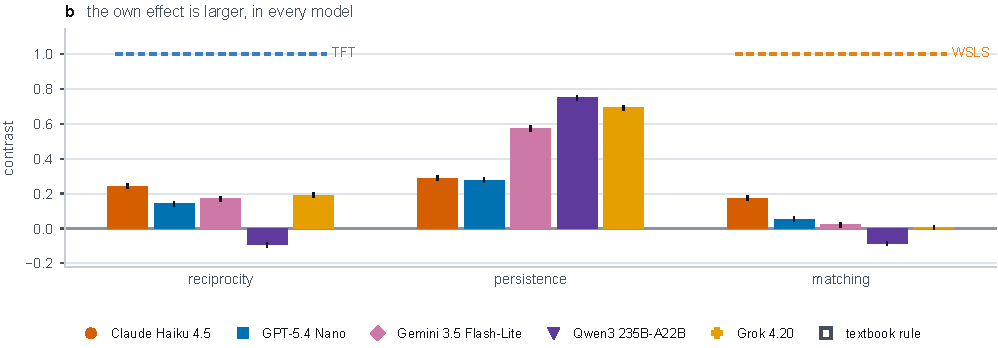
\includegraphics[width=\linewidth]{figures/f_strategy_space_b.pdf}\par
  \vspace{0.3cm}
  \raggedright
  \begin{itemize}
    \item \hb{Persistence} (own last move) beats \hb{reciprocity} (partner's
      last move) in every model
  \end{itemize}
  \note{With pXY = P(C | own move X, partner move Y) in the previous round: reciprocity
  = (pCC + pDC)/2 - (pCD + pDD)/2 (TFT = 1); persistence = (pCC + pCD)/2 -
  (pDC + pDD)/2; matching = (pCC + pDD)/2 - (pCD + pDC)/2 (WSLS = 1).
  Reciprocity is positive in four models and negative in Qwen; intervals are
  whole-dyad bootstrap. An unsupervised PCA recovers the same geometry.
  Caution: pCD - pDC equals persistence minus reciprocity, so it is not a
  reciprocity measure.}
\end{frame}

% ---------------------------------------------------------------------------
\begin{frame}{Remark}
  \begin{itemize}
    \item Payoff scale changes not only how often models cooperate,
      but also which rule their play resembles
    \bigskip
    \item As stakes grow, pooled LLM agents move away from AllD,
      evolutionary dynamics towards it
    \bigskip
    \item Agents respond more to their own moves than to their partner's
  \end{itemize}
\end{frame}

% ===========================================================================
% 4. Discussion and conclusions
% ===========================================================================
\begin{frame}{Why? Four candidate explanations}
  \begin{enumerate}
    \item Prompt text that does not scale\\
      {\mdseries\small narrative and persona}
    \medskip
    \item How numbers are represented\\
      {\mdseries\small sub-unit payoffs are rare and tokenised differently}
    \medskip
    \item Provider-specific post-training
    \medskip
    \item A distorted human stake response learned from text
  \end{enumerate}
  \vspace{0.4cm}
  {\centering Not mutually exclusive; the design cannot separate them\par}
  \note{Unlike human stake effects (modest, common direction, large stakes),
  here up to 0.636, opposite directions across models, concentrated at or below
  lambda = 1. Evidence: (1) consistent with the scale-dependent persona effects;
  (2) consistent with the change concentrating at or below lambda 1; (3)
  consistent with Qwen and Grok inverting the persona at every scale. The
  appendix proposes a design to test each. Limitations (backup): five models,
  one game, one template family; ten rounds limit strategy inference; no
  numeric-free condition, so a verbal baseline is the natural next step.}
\end{frame}

% ---------------------------------------------------------------------------
\begin{frame}{Conclusions}
  \begin{itemize}
    \item Payoff scale, formally irrelevant, systematically changes
      machine cooperation
    \medskip
    \item The effect is model-specific, language-dependent, and changes what
      persona prompts do
    \medskip
    \item It also changes which strategy the play resembles
    \medskip
    \item A cooperation rate is not a model trait: report the payoff scale and
      test \hb{scale sensitivity}
  \end{itemize}
  \vspace{0.3cm}
  \punch{Formal equivalences in the game are not automatically\\
    respected by the agents prompted to play it}
  \note{Implications: models of hybrid human-AI populations take an agent's
  cooperativeness as a parameter (Santos et al., Nature 2018; Han et al., Sci
  Rep 2013; Paiva et al., AAAI 2018); a rate partly set by the experimenter's
  units is not that parameter. Machine behaviour (Rahwan et al., Nature 2019):
  invariances give manipulations whose predicted effect is a stated number,
  zero. Paper: Han, Huynh, Duy-Minh et al., Payoff scaling shapes cooperation
  in LLM agents across languages, arXiv:2601.19082. Data and code: doi 10.5281/zenodo.23627009.}
\end{frame}

% ---------------------------------------------------------------------------
\begin{frame}{Thank you!}
  \centering
  {\titlefont\bfseries\fontsize{24}{28}\selectfont QUESTIONS?\par}
  \vspace{0.35cm}
  \begin{columns}[c]
    \column{0.52\textwidth}
    \raggedright
    {\scriptsize Payoff scaling shapes cooperation in LLM agents across languages\par}
    \vspace{0.2cm}
    {\mdseries\scriptsize
     T.\,A.\ Han, T.-K. Huynh, D.-S. Duy-Minh, T.-B. Cao, P.-H. Le, H.-D. Nguyen,
     P.-Q. Nguyen-Lam, M.-L. Nguyen-Vo, H.-P. Pham, P.-H. Pham, T.-K. Than,
     C.-N. Tran, H. Tran, G.-T. Tran-Le, A. Buscemi, L.\,H. Trang\par}
    \column{0.46\textwidth}
    \centering
    \begin{tabular}{@{}c@{\hspace{0.45cm}}c@{}}
      \href{https://arxiv.org/abs/2601.19082}{\qrcode[height=2.0cm]{https://arxiv.org/abs/2601.19082}} &
      \href{https://doi.org/10.5281/zenodo.23627009}{\qrcode[height=2.0cm]{https://doi.org/10.5281/zenodo.23627009}}\\[2pt]
      {\scriptsize Paper} & {\scriptsize Data and code}\\
      {\mdseries\tiny arXiv:2601.19082} & {\mdseries\tiny Zenodo}
    \end{tabular}
  \end{columns}
  \vspace{0.45cm}
  
\includegraphics[height=0.8cm]{logos/teesside.png}\hspace{0.35cm}%
  
\includegraphics[height=0.75cm]{logos/hcmut.png}\hspace{0.3cm}%
  
\includegraphics[height=0.8cm]{logos/hcmus.png}\hspace{0.3cm}%
  
\includegraphics[height=0.65cm]{logos/vnu.png}\hspace{0.3cm}%
  
\includegraphics[height=0.42cm]{logos/list.png}\par
  \vspace{0.35cm}
  {\small\href{mailto:t.han@tees.ac.uk}{\textcolor{DeepBlue}{\underline{t.han@tees.ac.uk}}}\par}
\end{frame}

% ===========================================================================
% Backup
% ===========================================================================
\appendix

\begin{frame}{Backup: how large is the departure?}
  \centering
  {\mdseries\small
  \renewcommand{\arraystretch}{1.2}
  \setlength{\tabcolsep}{4pt}
  \resizebox{\linewidth}{!}{%
  \begin{tabular}{lccccccc}
    \toprule
    & \multicolumn{2}{c}{cooperation} & & & & \multicolumn{2}{c}{Wald test}\\
    \cmidrule(lr){2-3}\cmidrule(lr){7-8}
    Model & min & max & \bfseries range & 95\% CI & $p_{\text{perm}}$ & $\chi^2_9$ & $p$\\
    \midrule
    Claude Haiku 4.5      & 0.371 & 0.452 & \bfseries 0.081 & [0.062, 0.135] & 0.0025 & 32.3 & $<$0.001\\
    GPT-5.4 Nano          & 0.438 & 0.680 & \bfseries 0.243 & [0.200, 0.290] & 0.0005 & 164.1 & $<$0.001\\
    Gemini 3.5 Flash-Lite & 0.682 & 0.872 & \bfseries 0.190 & [0.165, 0.240] & 0.0005 & 129.0 & $<$0.001\\
    Qwen3 235B-A22B       & 0.399 & 0.494 & \bfseries 0.095 & [0.068, 0.158] & 0.0005 & 96.9 & $<$0.001\\
    Grok 4.20             & 0.274 & 0.910 & \bfseries 0.636 & [0.588, 0.686] & 0.0005 & 1227.3 & $<$0.001\\
    \bottomrule
  \end{tabular}}}\par
  \vspace{0.5cm}
  \raggedright
  {\small Range over the ten scales, CI from 1,500 whole-dyad bootstrap draws.
  Permutation test shuffles the scale label among whole dyads (2,000 draws;
  0.0005 is the floor). Per-model logistic regression, scale as a 10-level
  factor, language and personas as covariates, SE clustered on the dyad.\par}
\end{frame}

\begin{frame}{Backup: variance decomposition}
  \centering
  {\mdseries\small
  \renewcommand{\arraystretch}{1.2}
  \begin{tabular}{lrrrrr}
    \toprule
    Term & Sum sq. & df & $F$ & $p$ & \% variance\\
    \midrule
    Model                    & 4.7871 & 4  & 187.27 & $<$0.001 & 45.4\\
    Language                 & 0.1599 & 4  & 6.25   & $<$0.001 & 1.5\\
    Payoff scale             & 0.6119 & 9  & 10.64  & $<$0.001 & 5.8\\
    Model $\times$ language  & 1.7901 & 16 & 17.51  & $<$0.001 & 17.0\\
    Model $\times$ scale     & 1.8910 & 36 & 8.22   & $<$0.001 & \bfseries 17.9\\
    Language $\times$ scale  & 0.3844 & 36 & 1.67   & 0.018    & 3.6\\
    Residual                 & 0.9202 & 144 &       &          & 8.7\\
    \bottomrule
  \end{tabular}}\par
  \vspace{0.5cm}
  \raggedright
  {\small Type-II ANOVA on the 250 model $\times$ language $\times$ scale cell means;
  the residual is the omitted three-way interaction. Without Grok the scale main
  effect is not significant ($F_{9,108} = 1.15$, $p = 0.33$).\par}
\end{frame}

\begin{frame}{Backup: persona effect by regime}
  \begin{columns}[c]
    \column{0.50\textwidth}
    \centering
    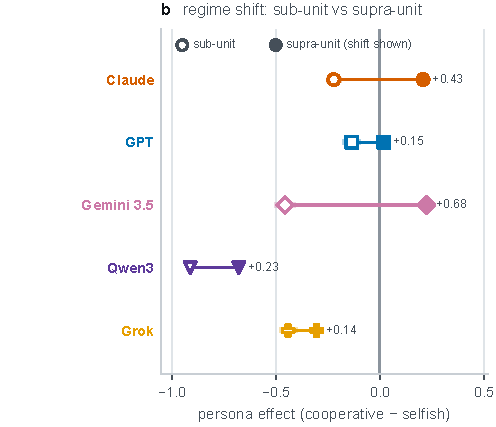
\includegraphics[width=\linewidth]{figures/f_persona_b.pdf}
    \column{0.49\textwidth}
    {\mdseries\scriptsize
    \renewcommand{\arraystretch}{1.25}
    \setlength{\tabcolsep}{2.5pt}
    \begin{tabular}{lccc}
      \toprule
      Model & $\lam \le 0.1$ & $\lam \ge 0.25$ & flip\\
      \midrule
      Claude  & $-0.222$ & $+0.207$ & yes\\
      GPT     & $-0.135$ & $+0.018$\textsuperscript{ns} & no\\
      Gemini  & $-0.456$ & $+0.224$ & yes\\
      Qwen3   & $-0.911$ & $-0.679$ & no\\
      Grok    & $-0.441$ & $-0.303$ & no\\
      \bottomrule
    \end{tabular}\par
    \medskip
    A flip needs both regime intervals (95\% dyad bootstrap) to exclude zero on
    opposite sides. GPT's supra-unit interval straddles zero: abolished, not
    reversed.\par}
  \end{columns}
\end{frame}

\begin{frame}{Backup: language effect by model}
  \begin{columns}[c]
    \column{0.58\textwidth}
    \centering
    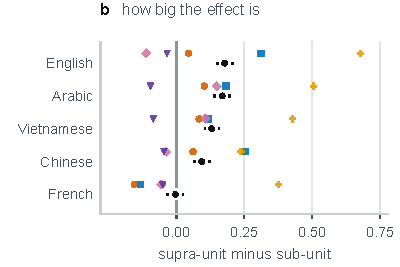
\includegraphics[width=\linewidth]{figures/f_language_b.pdf}
    \column{0.40\textwidth}
    {\small Supra-unit minus sub-unit cooperation. Black: five models pooled;
    markers: each model.\par
    \medskip
    The Arabic and Chinese templates state penalties but ask to maximise a
    reward: a prompt effect, not a cultural one.\par}
  \end{columns}
\end{frame}

\begin{frame}{Backup: baseline and corpus, full mix}
  \centering
  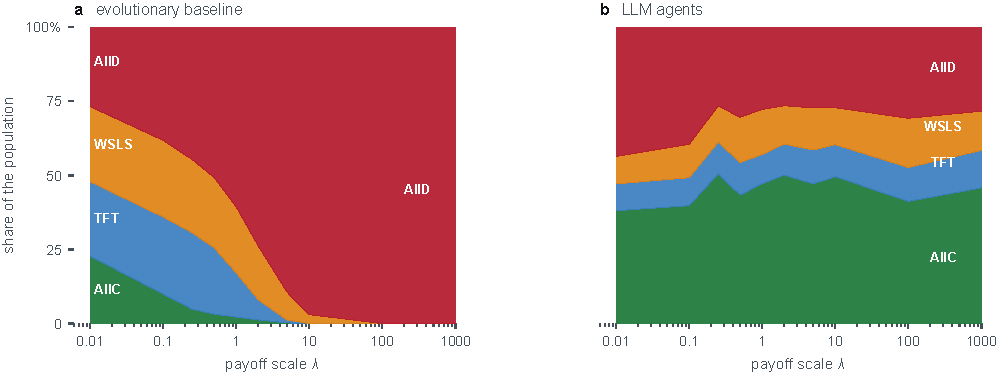
\includegraphics[width=\linewidth]{figures/f_egt_vs_llm_ab.pdf}\par
  \vspace{0.4cm}
  \raggedright
  {\small Left: stationary distribution of the evolutionary model
  ($Z = 100$, $\beta = 0.1$, $\varepsilon = 0.05$). Right: label shares in the
  corpus, pooled over models, languages and personas.\par}
\end{frame}

\begin{frame}{Backup: replicator dynamics ignore the scale}
  \centering
  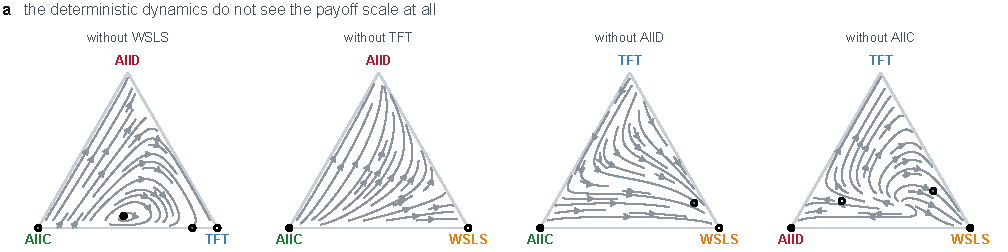
\includegraphics[width=\linewidth]{figures/f_simplex.pdf}\par
  \vspace{0.4cm}
  \raggedright
  {\small Normalised vector fields at $\lam = 0.01$ and $\lam = 1000$ agree to within
  $4 \times 10^{-14}$ over 2,000 random population states: the scale changes the
  speed, never the path.\par}
\end{frame}

\begin{frame}{Backup: robustness of the evolutionary direction}
  \centering
  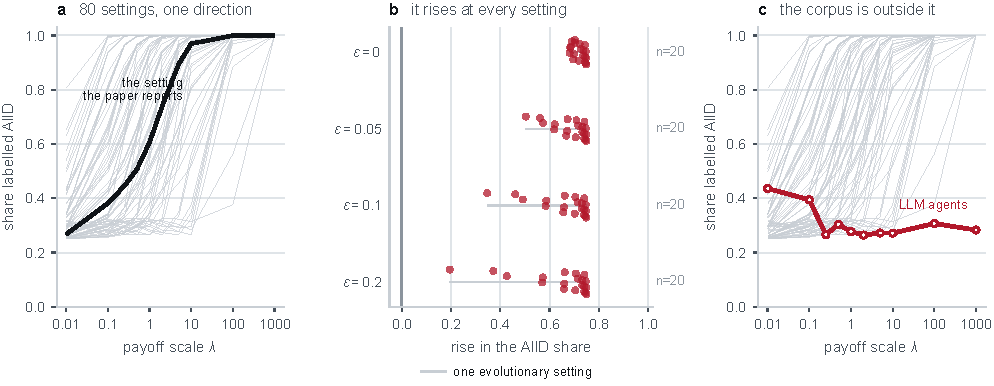
\includegraphics[width=\linewidth]{figures/f_robustness.pdf}\par
  \vspace{0.4cm}
  \raggedright
  {\small 80 settings, $Z \in \{50, 100, 200, 500\}$ $\times$
  $\beta \in \{0.01, 0.05, 0.1, 0.5, 1\}$ $\times$ $\varepsilon \in \{0, 0.05, 0.1, 0.2\}$:
  the stationary AllD share is higher
  at $\lam = 1000$ than at $\lam = 0.01$ in every one.\par}
\end{frame}

\begin{frame}{Backup: limitations}
  \begin{itemize}
    \item Five models, one repeated game, one family of prompt templates
    \medskip
    \item Language partly confounded with template wording
    \medskip
    \item Ten rounds limit strategy inference
    \medskip
    \item No numeric-free condition: next, a verbal baseline describing each
      outcome only by its rank
  \end{itemize}
\end{frame}

\begin{frame}{Image credits}
  \noindent{\mdseries\small Photographs from Wikimedia Commons.\par}
  \medskip
  \begin{itemize}\small\mdseries
    \item Robonaut and astronaut handshake: R.\ Markowitz, NASA, public domain
    \item Police interrogation room (movie set): nesnad, CC BY 3.0
    \item John von Neumann: courtesy of Los Alamos National Laboratory
      (free use with attribution)
    \item Prisoner's Dilemma sketch: Giulia Forsythe, CC0
    \item Tragedy and Comedy masks: Tim Green, CC BY 2.0
    \item Robot illustrations and model logos: the paper's Figure 1
    \item University logos: the universities' websites and Wikimedia Commons
  \end{itemize}
\end{frame}

\end{document}
